\lhead[\thepage]{CAPÍTULO \thechapter. PLANIFICACIÓN Y PRESUPUESTO}
\chead[]{}
\rhead[WepSIM: Simulador de procesador elemental con unidad de control microprogramada\leftmark]{\thepage}
\renewcommand{\headrulewidth}{0.5pt}

\lfoot[]{}
\cfoot[]{}
\rfoot[]{}
\renewcommand{\footrulewidth}{0pt}

%% This is an example first chapter.  You should put chapter/appendix that you
%% write into a separate file, and add a line \include{yourfilename} to
%% main.tex, where `yourfilename.tex' is the name of the chapter/appendix file.
%% You can process specific files by typing their names in at the 
%% \files=
%% prompt when you run the file main.tex through LaTeX.
\chapter{Planificación y presupuesto}
\label{ch:planning_and_budget}
\markboth{}{PLANNING AND BUDGET}

Este capítulo presenta una planificación detallada del proyecto (Sección \ref{sec:planning}, \textit{\nameref{sec:planning}}). Luego, explicamos los costes del proyecto (Sección \ref{sec:budget}, \textit{\nameref{sec:budget}}). Al final del capítulo, explicamos el entorno socio-económico del proyecto ({Section \ref{sec:socioeconomic_environment}, \textit{\nameref{sec:socioeconomic_environment}}}).

\section{Planificación}
\label{sec:planning}

Esta sección incluye la planificación completa del proyecto. En primer lugar, describimos la metodología de desarrollo de software utilizada. Después, detallamos la duración de cada fase del proyecto, indicando todos los tiempos en un gráfico de Gantt.

\subsection{Justificación de la Metodología}

Debido a sus características, hemos dividido nuestro proyecto en tres iteraciones:

\begin{itemize}
\item \textbf{Modelo hardware:} la primera iteración ha consistido en lograr el modelado del hardware que compone el procesador WepSIM. El objetivo de esta fase, ha sido lograr el modelado y funcionamiento básico de cada componente hardware por separado.

\item \textbf{Modelo software:} esta fase ha consistido en lograr el modelo software utilizado en la asignatura Estructura de computadores para la definición del juego de instrucciones y el lenguaje ensamblador. El objetivo de esta fase, ha sido lograr interpretar el juego de instrucciones definido y código ensamblador definidos por el usuario, generando la memoria de control y memoria principal en el orden correspondiente.

\item \textbf{Kernel del simulador:} esta fase ha consistido en lograr unir el modelo hardware y modelo software, realizando el kernel del simulador. El objetivo de esta fase, ha sido diseñar e implementar el kernel de simulador encargado de unir el modelo hardware y el modelo software, generando la simulación y la vista del simulador.
\end{itemize}

Era necesario contar con una metodología iterativa para desarrollar cada una de las fases de manera independiente para unirlas todas en la última etapa y obtener el producto final. Para ello, hemos analizado tres metodologías de desarrollo de software diferentes: Prototipado de software \cite{grimm1998}, el Modelo en Cascada \cite{hebert1983} y el Modelo en Espiral \cite{boehm1988}. El  Prototipado de Software no encaja muy bien en nuestro proyecto, puesto que requiere la construcción de un prototipo de sofware en poco tiempo. El Modelo en Cascada es un proceso de diseño secuencial, utilizado en procesos de desarrollo de software en el cual el progreso es visto como un flujo constante hacia abajo (como una cascada) a través de diferentes fases. El problema con esta metodología es que no permite iteraciones dentro del desarrollo del software. Finalmente, el Modelo en Espiral permitió dividir el proyecto en diferentes iteraciones. Este modelo, combina las fortalezas de los otros dos modelos (simplicidad y flexibilidad), utilizando además un proceso iterativo. Aunque este modelo es más lento que los dos anteriores, nos permitió aplicar diferentes iteraciones por lo que decidimos aplicarlo a todo el proceso.

\subsection{Ciclo de Vida}

El proceso de desarrollo del ciclo de vida del proyecto ha seguido el Modelo de ciclo de vida en Espiral \cite{boehm1988}. La Figura \ref{fig:spiral_model} muestra el Modelo en Espiral usando un esquema.

\begin{figure}[htbp]
 	\centering
 	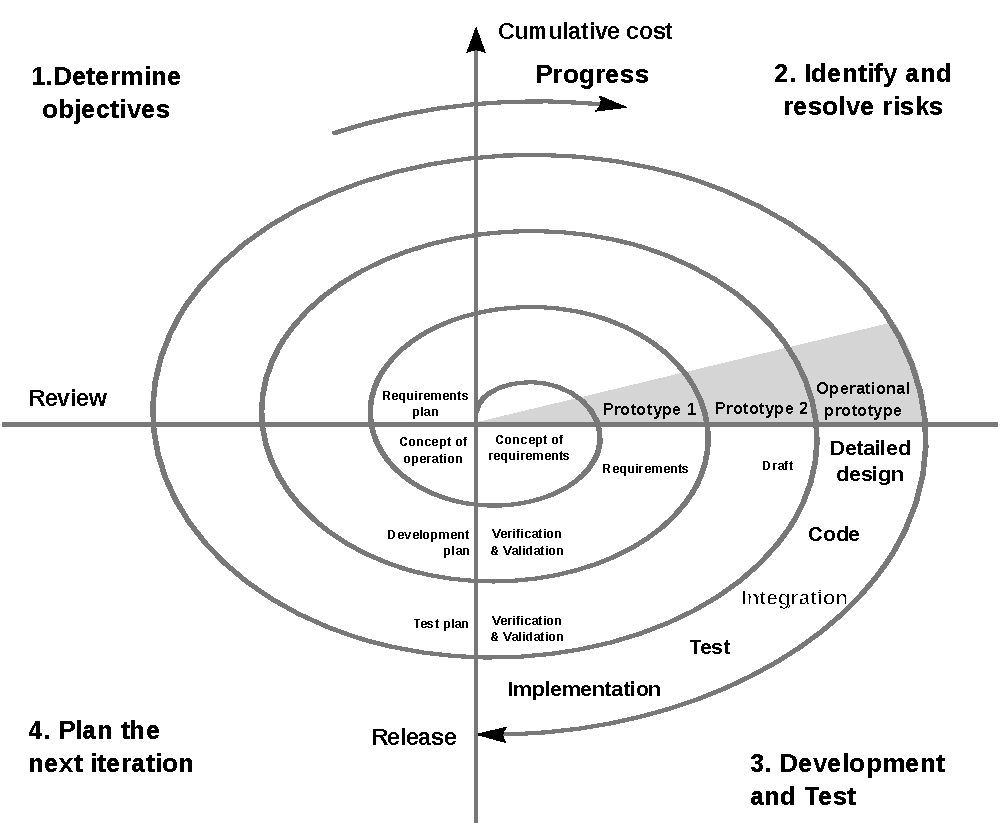
\includegraphics[width=12cm]{figures/spiral_model}
 	\caption{Modelo en Espiral (Boehm, 2000).}
	\label{fig:spiral_model}
\end{figure}

El modelo en Espiral tiene cuatro fases, que se repiten durante las diferentes iteraciones del modelo. Estas fases son:

\begin{itemize}
\item \textbf{Planificación} ('Determine objectives' en Figura \ref{fig:spiral_model}): Se reúnen los requisitos de los usuarios, se realiza un estudio de factibilidad del sistema y se determinan los objetivos de iteración.

\item \textbf{Análisis} ('Identify and resolve risks' en Figura \ref{fig:spiral_model}): Se realiza un análisis completo de los requisitos y se identifican los posibles riesgos. Esta fase termina con un diseño básico.

\item \textbf{Desarrollo y Pruebas}: Se lleva a cabo la implementación del código. Se realizan los casos de prueba y los resultados de la prueba.

\item \textbf{Evaluación} ('Plan the next iteration' in Figure \ref{fig:spiral_model}): 
Los clientes evalúan el software y proporcionan sus comentarios. En este caso, el estudiante intenta obtener la aprobación del supervisor. Esta es la \textit{tarea crítica} del ciclo de vida, ya que solo podemos pasar a la siguiente iteración del Modelo de ciclo de vida Espiral si esta tarea es aprobada.

\end{itemize}

Cada fase comienza con un objetivo de diseño y termina con el cliente (el supervisor) revisando el progreso hasta ahora. Como se explicó anteriormente, hemos dividido el desarrollo de software en tres iteraciones: modelo hardware, modelo software, y kernel del simulador. En la última iteración, el software completo debe someterse a pruebas exhaustivas para validar el simulador.

\subsection{Tiempo Estimado}

El gráfico de Gantt (Figura \ref{fig:gantt}) muestra todas las tareas realizadas durante el desarrollo del proyecto. El proyecto comenzó el 2 de noviembre de 2015 y finalizó el 30 de diciembre de 2016, lo que supone un total de casi 13 meses de trabajo (305 días laborables). Durante este tiempo, he trabajado de lunes a viernes, durante cuatro horas al día.

El diagrama de Gantt muestra todas las tareas realizadas en cada iteración del modelo de ciclo de vida espiral. Recuerde que las tres iteraciones fueron: Modelo hardware, Modelo software y kernel del simulador. Además de las tareas (fases) mencionadas anteriormente (Planificación, Análisis, Desarrollo y Prueba, y Evaluación), hemos incluido la tarea de Documentación al final de cada iteración. La tarea de documentación ha consistido principalmente en la redacción de este trabajo fin de grado.

\begin{figure}[htbp]
 	\centering
 	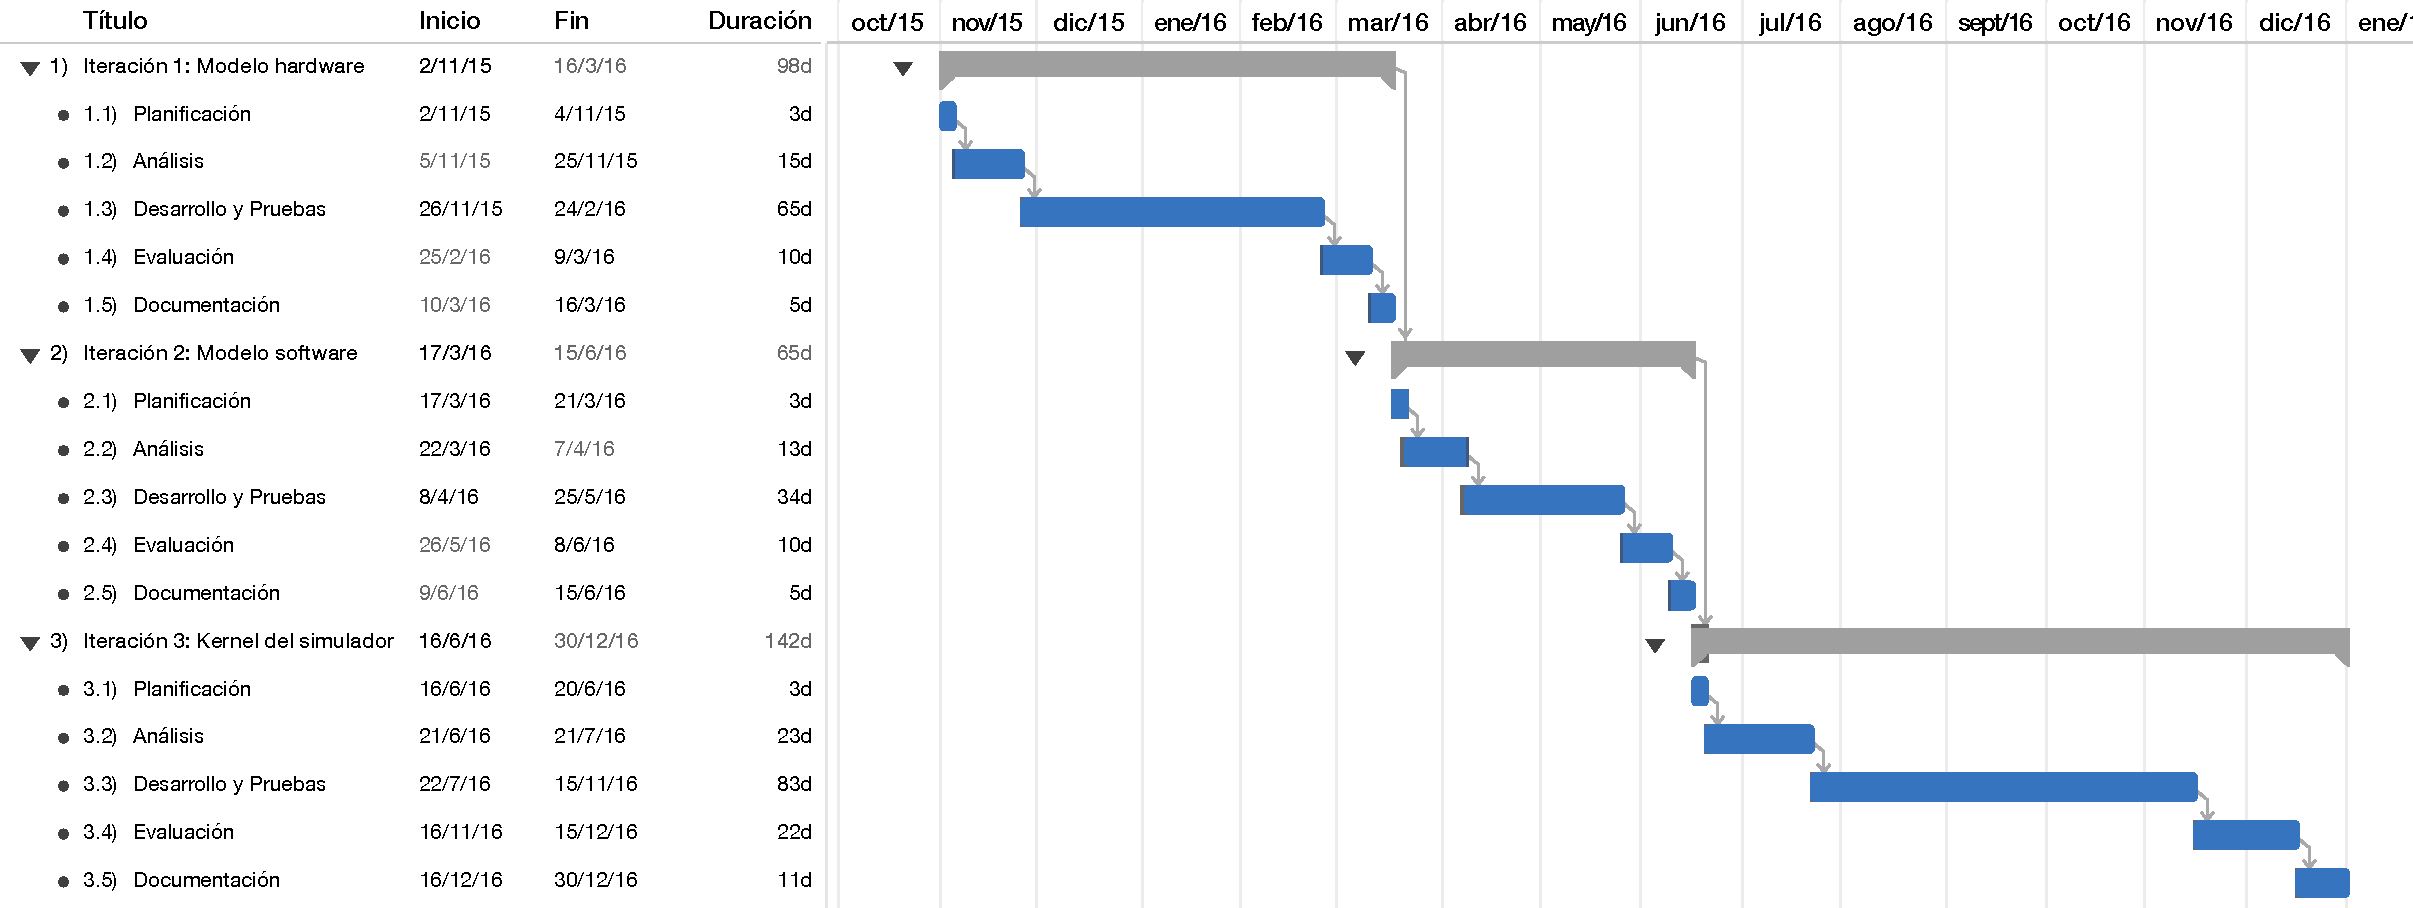
\includegraphics[width=16.5cm]{figures/ganttFuente}
 	\caption{Diagrama Gantt.}
	\label{fig:gantt}
\end{figure}

\section{Presupuesto}
\label{sec:budget}

Esta sección detalla el presupuesto general del proyecto. Por un lado, presentamos los costes del proyecto y, por otro lado, damos a conocer la oferta presentada al cliente.

\subsection{Coste del Proyecto}

La tabla \ref{tab:project_information} resume las principales características del proyecto, incluído el presupuesto total.

\begin{center}
\ra{1.2}
\begin{table*}[htbp]
\centering
\begin{tabular}{@{}p{3.5cm} p{9cm}@{}} 
\toprule
\multicolumn{2}{c}{\textbf{\textit{Información del Proyecto}}}\\
\midrule
\textbf{Título} 					& WepSIM: Simulador de procesador elemental con unidad de control microprogramada \\
\midrule
\textbf{Autor} 					& Javier Prieto Cepeda \\
\midrule
\textbf{Departamento} 				& Departamento de Informática \\
\midrule
\textbf{Fecha de inicio}				&2 de Noviembre de 2015 \\
\midrule
\textbf{Fecha de finalización}				& 30 de Diciembre de 2016 \\
\midrule
\textbf{Duración} 				& 13 meses \\
\midrule
\textbf{Ratio de costes indirectos} 	& 20 \% \\
\midrule
\textbf{Presupuesto total} 			& 51,860.96 \\
\bottomrule
\end{tabular}
\caption{Información del Proyecto.}
\label{tab:project_information}
\end{table*}
\end{center}

A continuación se desglosa el presupuesto total del proyecto.

\subsubsection{Costes Directos}

En esta parte se presentan los costos directos del proyecto. La Tabla \ref{tab:dhrc} muestra los costes directos causados por los costes de personal, sobre la base de la planificación presentada en la sección anterior. El tutor y el estudiante han desempeñado los siguientes roles:

\begin{itemize}

\item \textbf{Tutor:} Jefe de Proyecto.

\item \textbf{Estudiante:} Analista, Desarrollador, Tester.

\end{itemize} 

\begin{center}
\ra{1.2}
\begin{table*}[htbp]
\centering
\begin{tabular}{@{}p{3cm} R{3.5cm} R{2.2cm} R{2.4cm}@{}} 
\toprule
\textbf{Categoría} & \textbf{Coste por hora (\euro)} & \textbf{Horas} & \textbf{Total (\euro)} \\
\midrule
Jefe de Proyecto					& 60 						& 65			& 3,900 \\
Analista			 				& 35							& 269		& 9,415 \\
Desarrollador		 				& 35							& 523		& 18,305 \\
Tester		 					& 25							& 428		& 10,700 \\
\midrule
\textbf{\textit{Total}}			&							&			& \textbf{42,320.00}\\
\bottomrule
\end{tabular}
\caption{Costes de recursos humanos.}
\label{tab:dhrc}
\end{table*}
\end{center}

La tabla \ref{tab:dec} muestra los costes directos causados por la adquisición y uso del equipo. El coste amortizado, C, es calculado utilizando la siguiente formula:

\begin{equation}
  C = \frac{d \cdot c \cdot u}{D}
\label{eq:costs}
\end{equation}

Donde:

\begin{itemize}

\item \textbf{C:} Coste amortizado. Es equivalente al valor amortizado.

\item \textbf{d:} Tiempo que el equipamiento ha sido utilizado.

\item \textbf{c:} Coste del equipamiento. 

\item \textbf{u:} Dedicación al proyecto. Porcentaje del tiempo que el equipamiento ha sido utilizado.

\item \textbf{D:} Periodo de amortización del equipamiento.

\end{itemize}

\begin{center}
\ra{1.2}
\begin{table*}[htbp]
\centering
\begin{tabular}{@{}p{2.5cm} C{1.8cm} C{2.1cm} C{2.1cm} C{2.7cm} C{2.3cm}@{}} 
\toprule
\textbf{Concepto} & \textbf{Coste, c (\euro)} & \textbf{Dedicación, u (\%)} & \textbf{Dedicación, d (meses)} & \textbf{Amortización, D (meses)} & \textbf{Coste amortizado, C (\euro)}\\
\midrule
Desktop \acrshort{pc}		 			& \multicolumn{1}{r}{799.99}		& \multicolumn{1}{r}{100}		& \multicolumn{1}{r}{13} 		& 	\multicolumn{1}{r}{36}	& 	\multicolumn{1}{r}{288.89} \\
Laptop 						& \multicolumn{1}{r}{529.99} 	& \multicolumn{1}{r}{25}			& \multicolumn{1}{r}{13} 		& 	\multicolumn{1}{r}{36}	& 	\multicolumn{1}{r}{47.85} \\
\acrshort{arcos} Mirlo					& \multicolumn{1}{r}{1979.99}	& \multicolumn{1}{r}{50}			& \multicolumn{1}{r}{7} 		& 	\multicolumn{1}{r}{60}	& 	\multicolumn{1}{r}{115.50} \\
Impresora						& \multicolumn{1}{r}{79.99}		& \multicolumn{1}{r}{5}			& \multicolumn{1}{r}{4}		& 	\multicolumn{1}{r}{60}	& 	\multicolumn{1}{r}{0.27} \\
\midrule
\textbf{\textit{Total}}		&			&			& 			& &  \multicolumn{1}{r}{\textbf{452.50}}\\
\bottomrule
\end{tabular}
\caption{Costes de equipamiento.}
\label{tab:dec}
\end{table*}
\end{center}

Además, el equipo presentado en la Tabla \ref{tab:dec} es detallado a continuación:

\begin{itemize}

\item \textbf{Desktop \acrshort{pc}:} All in One - Asus Z220ICUK, 21.5'', i5-6400T, 8GB, 1TB)		

\item \textbf{Laptop:} Toshiba L50D-C-19D, A10-8700P, 8GB \gls{ram} and 1TB.

\item \textbf{\acrshort{arcos} Mirlo:} Servidor utilizado por el grupo de investigación \acrshort{arcos}. 32GB \gls{ram} and eight i7 processors of 2.67GHz each.

\item \textbf{Impresora:} Brother DCP-1510.

\end{itemize}

Otros costes directos se muestran en la Tabla \ref{tab:odc}. Estos costes consisten en material de oficina, un tóner para la impresora y el abono transporte mensual. El material de oficina incluye: lápices, bolígrafos, cuadernos, papel, tipex y marcadores.



\begin{center}
\ra{1.2}
\begin{table*}[htbp]
\centering
\begin{tabular}{@{}p{5cm} R{3.5cm}@{}} 
\toprule
\textbf{Concepto} & \textbf{Coste (\euro)} \\
\midrule
Material de oficina				& 112.98				\\
Toner (x1) 			 			& 71.99				\\
Abono transporte (x13) 		& 260				\\
\midrule
\textbf{\textit{Total}}		&	\textbf{444.97}  	\\
\bottomrule
\end{tabular}
\caption{Otros costes directos.}
\label{tab:odc}
\end{table*}
\end{center}

\subsubsection{Resumen de Costes}

La Tabla \ref{tab:cs} muestra el resumen completo de los costes del proyecto. Los costes indirectos (20\% de los costes directos) consisten en las facturas de electricidad y agua, teléfono, acceso a internet, etc.

\begin{center}
\ra{1.2}
\begin{table*}[htbp]
\centering
\begin{tabular}{@{}p{5cm} R{5cm}@{}} 
\toprule
\multicolumn{2}{c}{\textbf{\textit{Resumen de costes}}}\\
\midrule
\textbf{Recursos humanos} 				& 42,320.00 \\
\textbf{Equipamiento} 						& 452.50 \\
\textbf{Otros costes directos} 				& 444.97 \\
\textbf{Costes indirectos}					& 8,643.49 \\
\midrule
\textbf{\textit{Presupuesto total}}			& \textbf{51,860.96} \\
\bottomrule
\end{tabular}
\caption{Resumen de costes.}
\label{tab:cs}
\end{table*}
\end{center}

El presupuesto total de este proyecto asciende a \textbf{51,860.96 \euro \ (cincuenta y uno mil ochocientos sesenta euros y noventa y seis céntimos)}.

\subsection{Oferta de Proyecto Propuesta}

La Tabla \ref{tab:offer} una propuesta de oferta detallada. Esta oferta incluye los riesgos estimados (20\%), los beneficios esperados (15\%), y el Impuesto de Valor Agregado (\gls{iva}), que corresponde al 21\% \cite{iva2012}. Después de aplicar todos estos conceptos, la cantidad final para este proyecto en caso de venta a un cliente de terceros es \textbf{86,597.43 \euro \ 
(Ochenta y seis mil quinientos noventa y siete euros y cuarenta y tres céntimos)}.

\begin{center}
\ra{1.2}
\begin{table*}[htbp]
\centering
\begin{tabular}{@{}p{2.5cm} R{2.6cm} R{3.1cm} R{3.5cm}@{}} 
\toprule
\multicolumn{4}{c}{\textbf{\textit{Oferta propuesta}}}\\
\midrule
\textbf{Concepto} & \textbf{Incremento (\%)} & \textbf{Valor Parcial (\euro)} & \textbf{Coste agregado (\euro)} \\
\midrule
Costes del proyecto				& - 			& 51,860.96		& 51,860.96 \\
Riesgos			 				& 20			& 10,372.19		& 62,233.15 \\
Beneficios		 				& 15			& 9,334.97		& 71,568.13 \\
IVA		 					& 21			& 15,029.31		& 86,597.43 \\
\midrule
\textbf{\textit{Total}}		&			&			& \textbf{86,597.43}\\
\bottomrule
\end{tabular}
\caption{Oferta propuesta.}
\label{tab:offer}
\end{table*}
\end{center}

\section{Entorno Socio-Económico}
\label{sec:socioeconomic_environment}

Como se ha comentado en capítulos anteriores, WepSIM puede apoyar la enseñanza en Estructura y Arquitectura de Computadores. Esto significa que los profesores de estas asignaturas pueden utilizar esta herramienta como refuerzo en las explicaciones del temario para mostrar de forma visual y práctica a los alumnos el comportamiento de un procesador elemental. Además, sirve para que los alumnos puedan desarrollar las prácticas de estas asignaturas sin la necesidad de utilizar diferentes herramientas, evitando la pérdida de tiempo que esto supone y permitiendo a los alumnos dedicar el mayor tiempo posible a la realización de los ejercicios.

Además, debido al diseño realizado de este simulador, WepSIM permite la especificación tanto de diferentes juegos de instrucciones como de diferentes modelos hardware. Esto supone un gran avance  en el área docente, puesto que permite el uso de una misma herramienta para la enseñanza y simulación de diferentes dispositivos. Anteriormente se invertía mucho dinero para que los alumnos pudieran realizar prácticas con diferentes tipos de procesadores, ya que se debían de adquirir los diferentes componentes hardware necesarios para la realización de las prácticas. Con WepSIM este concepto cambia, puesto que modelando el comportamiento del computador deseado, puede ser utilizado para diferentes tipos de prácticas, evitando costes de adquisición y mantenimiento y permitiendo una mayor variedad de opciones a la hora de diseñar las prácticas.

Gracias al uso de este simulador en el ámbito docente, se puede mostrar el impacto energético que supone una programación eficiente. Esto es debido a que WepSIM es un simulador de microprogramación y programación en ensamblador, pudiendo hacer visible el coste a bajo nivel de unas malas prácticas de programación. El objetivo, es concienciar a los alumnos de la importancia que tiene la optimización y eficiencia en el uso de los recursos de un computador, puesto que uno de los retos de la comunidad científica es diseñar sistemas cada vez más eficientes energéticamente.
